\documentclass{article}

% set font encoding for PDFLaTeX or XeLaTeX
\usepackage{ifxetex}
\ifxetex
  \usepackage{fontspec}
\else
  \usepackage[T1]{fontenc}
  \usepackage[utf8]{inputenc}
  \usepackage{lmodern}
  \usepackage{graphicx}
\fi

% used in maketitle
\title{Caracterisiticas,limitaciones y bondades de jupyter notebook}
\author{Ramses Pacheco Ortiz}
\date{8 de febrero del 2018}
% Enable SageTeX to run SageMath code right inside this LaTeX file.
% documentation: http://mirrors.ctan.org/macros/latex/contrib/sagetex/sagetexpackage.pdf
% \usepackage{sagetex}

\begin{document}
\maketitle

\section{Objetivos}
Los principales objetivos en está 2da actividad es conocer el manejo del lenguage de programacion en python asi como utlizar sus herrmientas basicas para el uso adecuado y correcto para aprovechar al maximo la aplicacion utilizada.


\section{características}

\begin{itemize}
\item
Python es un lenguaje muy simple, por lo que es muy fácil iniciarse en este lenguaje. El pseudo-código natural de Python es una de sus grandes fortalezas.

\item
Debito a la naturaleza de Python de ser Open Suorce; ha sido modificado para que pueda funcionar en diversas plataformas (Linux, Windows, Macintosh, Solaris, Amiga, PlayStation, Sharp Zaurus, Windows CE y PocketPC).

Al ser Open Source es gratuito.

\item
Python contiene una gran cantidad de librerías, tipos de datos y funciones incorporadas en el propio lenguaje, que ayudan a realizar muchas tareas comunes sin necesidad de tener que programarlas desde cero.

Las librerías pueden ayudar a hacer varias cosas como expresiones regulares, generación de documentos, evaluación de unidades, pruebas, procesos, bases de datos.

\item
Python tiene una sintaxis muy visual, gracias a que maneja una sintaxis identada (con márgenes), que es de caracter obligatorio. Para separar los bloques de código en Python se debe tabular hacia dentro. Esto ayuda a que todos los programadores adopten las mismas notaciones y que los programas hechos en Python tengan un aspecto muy similar.






\section{Desarrollo}
\subsection{exportacion de datos}
Pandas es una librería de python destinada al análisis de datos, que proporciona unas estructuras de datos flexibles y que permiten trabajar con ellos de forma muy eficiente.


Lo primero que debemos hacer es importar la libreria de Pandas como:

\begin{figure}[h!]
  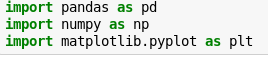
\includegraphics[width=\linewidth]{1.png}
 \end{figure}


\subsection{Actividades realizadas}

Despues de que seguimos una serie de pasos,para familiriazarnos con el nuevo lenguage de programacion python,realizamos una serie de actividades y representaciones graficas de los datos de una ciudad que nostros esocogimos  anteriormente,las activdades fueron las siguintes:

Primero elaboramos una grafica de las rapideces de los vientos y rafagas con los datos,utilizando el codigo de python para graficar y poder editar estás,por ejemplo:
\item  para graficar las dos funciones de rapideces en la misma grafica \ref{fig:grafica1}

Se utilizo: plt.fugre(): df1.plot(): plt legend(loc='best')

\item Para ponerle titulo ala grafica se utilizo lo siguiente:

plt.title("el nombre de la grafica")

\begin{figure}[ht!]
 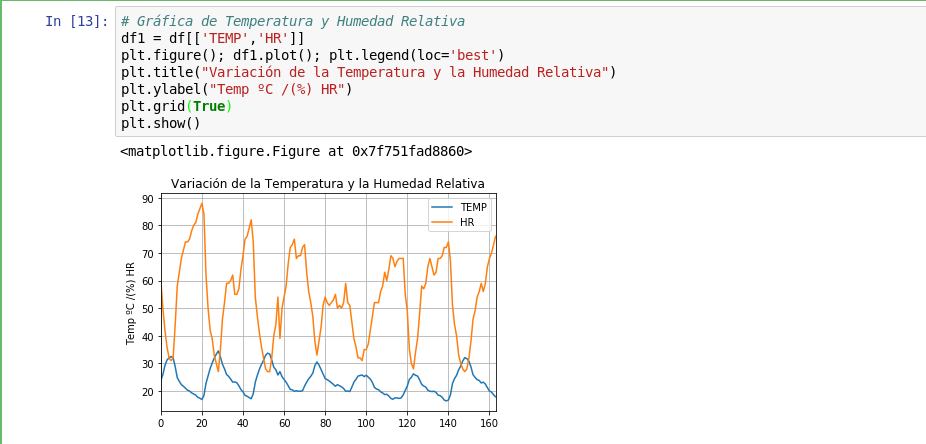
\includegraphics[width=\linewidth]{2.png}
 \caption{Rapideces de los vienos y rafagas}
 \label{fig:grafica1}
 \end{figure}

\item En esta grafica \ref{fig:grafica2} observamos la direccion del viento con respecto al tiempo y observamos que,los vientos dominantes son abundantes por esta ciudad el mas alto fue de 355 aprox.

\begin{figure}[ht!]
 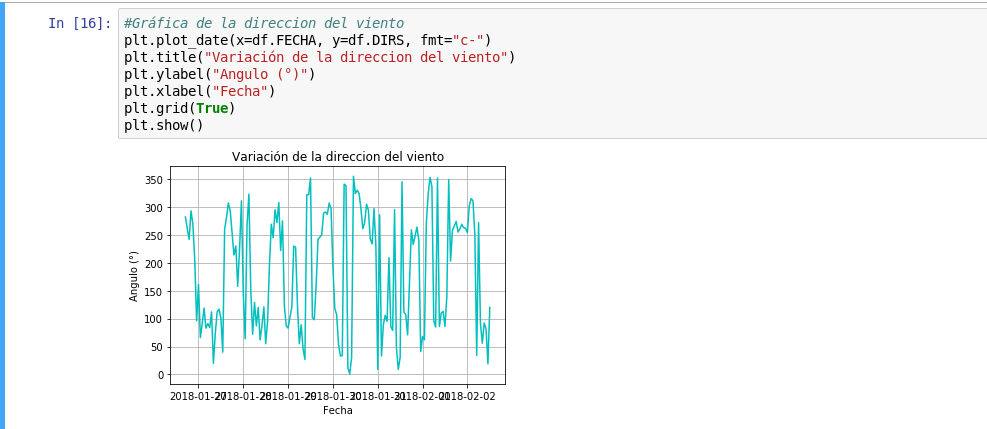
\includegraphics[width=\linewidth]{3.png}
  \caption{direccion del viento}
 \label{fig:grafica2}
 \end{figure}

\item La siguiente actividad realizada fue hacer una grafica \ref{fig:grafica3} de radiacion contra el tiempo,con el codigo siguiente:

 \begin{itemize}
 \item
 plt.x ó y label son para escribir en los ejes de las graficas
 \item
 fmt"es para cambiar el color y el estilo de liena de la grafica.
 \item
 x=df.FECHA , y=df.RADSOL "son para graficar esos datos en los ejes correspondintes"

 \end{itemize}

 \item
en la grafica \ref{fig:4} se puedes observa el comportamiento de la radiacion solar
\begin{itemize}
\item el compartameinto dela grafica solar es muy paracido por lo tanto,el clima se mantuvo muy parecido con excepcion de algunos casos.
\end{itemize}
\item realizamos la dirferencia de temperatura entre la maxima y minima para calcular el lapśo de temperatura diaria. Esto se muestra en la grafica \ref{fig:5}



\begin{figure}[ht!]
 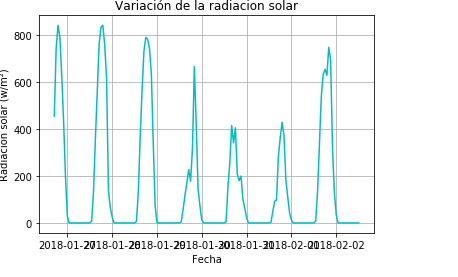
\includegraphics[width=1\linewidth]{5.png}
 \caption{Radiación solar}
 \label{fig:4}
 \end{figure}

 \begin{figure}[ht!]
 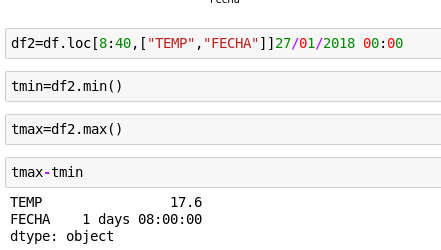
\includegraphics[width=1\linewidth]{6.png}
 \caption{Diferencia de temperaturas}
 \label{fig:5}
 \end{figure}

 \item
por ultimo usamos una funcion de discribe,mostrando el análisis exploratorio de datos, que resuma el sitio estudiado,mostrado en la grafica \ref{fig:6}


 \begin{figure}[ht!]
 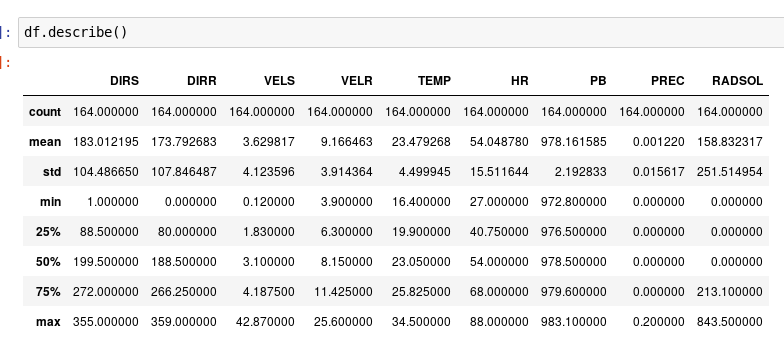
\includegraphics[width=1\linewidth]{8.png}
 \caption{Funcion describe}
 \label{fig:6}
 \end{figure}

\end{itemize}




\section{Bondades}
pandas es muy buen sitio para tratar ciertos tipos de datos como los siguiente:



\begin{itemize}

\item
Datos tabulares con columnas de tipo heterogéneo, como en una tabla SQL o en una hoja de cálculo de Excel
\item
Datos ordenados y desordenados (no necesariamente frecuencia fija).

\item
Datos matriciales arbitrarios (homogéneamente tipados o heterogéneos) con etiquetas de fila y columna

\item
Cualquier otra forma de conjuntos de datos observacionalesy estadísticos. Los datos en realidad no necesitan ser etiquetados para ser colocados en una estructura de datos de pandas

\end{itemize}

\section{Mas sobre panda}
\begin{itemize}
\item
Las dos estructuras de datos principales de pandas, Series (1-dimensional) y DataFrame (2-dimensional), manejan la gran mayoría de casos de uso típicos en finanzas, estadísticas, ciencias sociales y muchas áreas de la ingeniería.
\item
Pandas se basa en NumPy y está pensado para integrarse bien en un entorno informático científico con muchas otras bibliotecas de terceros.

\item
Estas son solo algunas de las cosas que los pandas hacen bien:


Manejo sencillo de datos faltantes (representados como NaN) en coma flotante, así como en datos no flotantes

\item
Mutabilidad de tamaño: las columnas se pueden insertar y eliminar de DataFrame y objetos dimensionales superiores
\item
Alineación de datos automática y explícita: los objetos se pueden alinear explícitamente con un conjunto de etiquetas, o el usuario puede simplemente ignorar las etiquetas y dejar que Series, DataFrame, etc.

\item
Grupo potente y flexible por funcionalidad para realizar operaciones de combinación de aplicación dividida en conjuntos de datos, para agregar y transformar datos.

\item
Corte inteligente basado en etiquetas, indexación elegante y subconjunto de grandes conjuntos de datos.

\item
Etiquetado jerárquico de ejes (es posible tener etiquetas múltiples por marca).

\end{itemize}

\section{Apendice }


1.-¿Cuál es tu primera impresión de Jupyter Notebook?


Creo que es muy paracida a drive ,pero si puedes hacer muchas mas cosas con jupyter


2.-¿Se te dificultó leer código en Python?


A lo primero ya que se me hacia un poco diferente los codigos comparados con fortran.pero depues  ya me acostumbre y supe lo que signficaba.


3.-¿En base a tu experiencia de programación en Fortran, que te parece el entorno de trabajar en Python?

Muy bien ya que la paltaforma es muy ordenada y mucho mas sencilla de usar y detectar errores


4.- A diferencia de Fortran, ahora se producen las gráficas utilizando la biblioteca Matplotlib. ¿Cómo fue tu experiencia?.


bien creo que es mas sencillo entender el codigo, mas facil de escribirlo y manipularlo

5.- En general, ¿qué te pereció el entorno de trabajo en Python?

bien es mucho mas secillo que en fortran en todo aspecto ya sea, en plataforma ,codigo fuente,lenguage de programacion,etc.


6.-Qué opinas de la actividad? ¿Estuvo compleja? ¿Mucho material nuevo? ¿Que le faltó o que le sobró? ¿Qué modificarías para mejorar?

Me parecio muy buena actividad ,pero si fue material un poco nuevo
7.-¿Comentarios adicionales que desees compartir?







\end{document}
